\documentclass{beamer}
\mode<presentation>
\usepackage{amssymb,textcomp}
%\usepackage{beamerthemesplit}
\usepackage{beamerthemeJuanLesPins}
\usepackage{verbatim}
\usepackage{algorithm2e}
\usefonttheme{serif}
\title{Unidad I: Teor\'ia de Aproximaci\'on.}
\author{Jos\'e Luis Ram\'irez B.}
\date{\today}

\begin{document}

\frame{\titlepage}

\frame{\tableofcontents}

\section{Introducci\'on}
\begin{frame}[fragile]
  \frametitle{Motivaci\'on.} 
  \begin{itemize}
    \item<1-> La gran mayor\'ia de los modelos matem\'aticos que describen procesos f\'isicos no pueden resolverse anal\'iticamente.
    \item<2-> En una situaci\'on pr\'actica, un problema matem\'atico deriva de un fen\'omeno f\'isico sobre el cual se han hecho algunas suposiciones para simplificarlo y poderlo representar matem\'aticamente.
    \item<3-> Una vez formulado el problema, deben dise\~narse m\'etodos num\'ericos para resolver el problema. La selecci\'on o construcci\'on de los algoritmos apropiados cae propiamente dentro del terreno del An\'alisis Num\'erico.
  \end{itemize}    
\end{frame}
%%%%%
\section{Teor\'ia de Errores y Aproximaci\'on.}
\begin{frame}[fragile]
  \frametitle{Teor\'ia de Errores y Aproximaci\'on.}
  El an\'alisis num\'erico proporciona m\'etodos computacionales para el estudio y soluci\'on de problemas matem\'aticos. Debido a que muchos c\'alculos son realizados en computadores digitales, es conveniente la discusi\'on para la implementaci\'on de los m\'etodos num\'ericos como programas de computador..
\end{frame}
%%%%%
\begin{frame}[fragile]
  \frametitle{Teor\'ia de Errores y Aproximaci\'on.}
\begin{itemize}
  \item La aparici\'on de computadores ha hecho posible la soluci\'on de problemas, que por su tama\~no antes eran
  excluidos.
  \item<2-> Desafortunadamente los resultados son afectados por el uso de la Aritm\'etica de Precisi\'on Finita.
  \item<3-> Esperamos tener siempre expresiones verdaderas como $2+2=4$, $3^2=9$, $(\sqrt{5})^2 = 5$, pero en la aritm\'etica de precisi\'on finita $\sqrt{5}$ no tiene un solo n\'umero fijo y finito, que lo representa.
  \item<4-> En el computador se le da un valor aproximado cuyo cuadrado no es exactamente 5, aunque con toda probabilidad estar\'a lo bastante cerca a \'el para que
  sea aceptable.
\end{itemize}  
\end{frame}
%%%%%
\begin{frame}
  \frametitle{Teor\'ia de Errores y Aproximaci\'on.}
  Un m\'etodo num\'erico es un procedimiento mediante el cual se obtiene, de manera aproximada, la soluci\'on de ciertos problemas. Los resultados num\'ericos est\'an influenciados por muchos tipos de errores, los cuales pueden ser catalogados a  grandes rasgos en tres tipos b\'asicos:
  
  \begin{itemize}
   \item<2-> \textbf{Errores inherentes} que existen en los valores de los datos de entrada, ya sea causados por incertidumbre o por la naturaleza necesariamente aproximada de la representaci\'on.
    \item<3-> \textbf{Errores de discretizaci\'on} (llamados tambi\'en de truncamiento) que surgen al reemplazar procesos l\'imites por su resultado antes de alcanzar tal l\'imite.
    \item<4-> \textbf{Errores de redondeo} que se originan al utilizar una aritm\'etica que involucra n\'umeros con un n\'umero finito de d\'igitos.
  \end{itemize}
\end{frame}
%%%%%%
\frame
{
  \frametitle{Errores Absolutos y Relativos.}


  Sea $x$ el valor exacto de un n\'umero real y $\tilde{x}$ el valor aproximado. Contemplando todos los posibles errores, la relaci\'on entre el resultado exacto y el aproximado es:
$$
x = \tilde{x}+E
$$

\uncover<2->{
Se define el error absoluto y se denota $E_a$ como la diferencia $x-\tilde{x}$, y se expresa siempre en valor absoluto.
\begin{block}{}
 $$
 E_a = |x-\tilde{x}|
 $$
\end{block}}
}
%%%%
\frame{
\frametitle{Forward and Backward Error}
\begin{itemize}
   \item Sea $x$ un n\'umero real y $f:\mathbb{R}\to\mathbb{R}$ una funci\'on. Si $\tilde{y}$ es un 
n\'umero real que es una aproximaci\'on a $y=f(x)$, entonces el error hacia adelante (Forward) en 
$\tilde{y}$ es la diferencia $\Delta y=\tilde{y}-y$.
\item<2-> Sea $x\in \mathbb{R}$ y $f:\mathbb{R}\to\mathbb{R}$ una funci\'on. Sup\'ongase que 
$\tilde{y}$ es una aproximaci\'on a $y=f(x)$ y $\tilde{y}$ est\'a en el rango de $f$, es decir, 
$\tilde{y}=f(\tilde{x})$ para alg\'un $\tilde{x}$, entonces la cantidad $\Delta x=\tilde{x}-x$ es 
el error hacia atr\'as (Backward) en $\tilde{y}$.
\end{itemize}
}
%%%
\frame{
\frametitle{Forward and Backward Error}
\underline{Ejemplo:}

Sup\'ongase que se desea calcular $y=\sqrt{2}$ y se obtiene $\tilde{y}=1.4$, entonces:
\begin{itemize}
   \item<2-> Forward Error: $|\Delta y|=|\tilde y - y|=|1.4-1.4142\ldots|\approx 0.0142\ldots$
   \item<3-> Backward Error: N\'otese que $\sqrt{1.96}=1.4$, entonces  $|\Delta 
x|=|\tilde{x}-x|=|1.96-2|=0.04$
\end{itemize}
}
%%%%
\frame
{\frametitle{Errores Absolutos y Relativos.}

Una debilidad de esta definici\'on es que la magnitud del error verdadero depende de la escala. 
\begin{itemize}
 \item<2-> Por ejemplo podemos medir una barra en cent\'imetros o en metros. Si la longitud exacta de la barra es $1m$ 
y por la medici\'on se obtiene $99cm$, 
\begin{enumerate}
 \item<3-> $E_a = 100 - 99 = 1$, si usamos cent\'imetros.
 \item<4-> $E_a = 1.00 - 0.99 = 0.01$, si usamos metros.
\end{enumerate}
\end{itemize}

\uncover<5->{Esta es la raz\'on por la que se define el error relativo.}
}
%%%%
\frame
{
  \frametitle{Errores Absolutos y Relativos.}
  Al cociente entre el error absoluto $E_a$ y el valor real $x$ se le denomina error relativo y se denota por $E_r$. Se 
expresa tambi\'en en valor absoluto, es decir:
\uncover<2->{
\begin{block}{}
 $$
 E_r = \frac{|E_a|}{|x|}=\frac{|x-\tilde{x}|}{|x|}
 $$
\end{block}}
}
%%%%%
\begin{frame}
\frametitle{Errores Absolutos y Relativos.}
\begin{itemize}
 \item<1-> Es preferible trabajar con errores relativos pues se toma en cuenta las magnitudes de los
 n\'umeros con los que se est\'a trabajando. 
 \item<2->El uso del error absoluto tiene sentido s\'olamente si se tiene informaci\'on a priori de estas magnitudes.
 \item <3-> De este modo un valor aproximado puede ser expresado de la siguiente manera en funci\'on del error relativo cometido y el valor real:
 \begin{block}{}
 $$
 E_r = \frac{E_a}{x} = \frac{\tilde x - x}{x}  \Rightarrow xE_r = \tilde x -x \Rightarrow x+xE_r =\tilde x \Rightarrow
 \tilde x = x(1+E_r)
 $$ 
 \end{block}
\end{itemize}
\end{frame}
%%%%
\frame
{
  \frametitle{Cifras Significativas.}
  Se dice que el n\'umero $\tilde{x}$ aproxima al n\'umero $x$ con $t$ d\'igitos (o cifras) significativas, si $t$ es el n\'umero m\'as grande no negativo para el cual:
$$
E_r < 0.5\times10^{-t}\Rightarrow \frac{|x-\tilde{x}|}{|x|}<0.5\times10^{-t}
$$

\uncover<2->{
\begin{block}{Ejemplo:}
Sea $\tilde{x}=3.1416$ una aproximaci\'on al valor $\pi$, y $x=3.1415927$ una mejor aproximaci\'on.
\begin{eqnarray}
 E_a &=& |x - \tilde{x}| = |3.1415927-3.1416| = 0.0000073\nonumber\\
 E_r &=& \frac{E_a}{|x|} =\frac{0.0000073}{3.1415927} = 0.0000023237\nonumber\\
 t&<&-\frac{\ln(2E_r)}{\ln(10)} = 5.3329\nonumber
\end{eqnarray}

\end{block}
}
}
%%%%%%%%
\begin{frame}
  \frametitle{Cifras Significativas.}
  \textbf{Ejemplo:} Hallar el rango de aproximaciones con 4 cifras significativas para $x = 1000$
\uncover<2->{
  \begin{flalign}
  \nonumber & \frac{|1000-\tilde x|}{|1000|}<5\times 10^{-4} \Rightarrow |1000 - \tilde x|<5\times 10^{-1}\Rightarrow
  |1000 -\tilde x|<0,5\\
  \nonumber  & -0.5 < 1000 - \tilde x < 0.5 \Rightarrow  999.5 < \tilde x < 1000.5\\
  \nonumber & \mbox{Rango }=(999.5;  1000.5) 
  \end{flalign}
  }
  \uncover<3->{
    \begin{block}{Observaci\'on}
      Las cifras significativas dan una idea de la exactitud en t\'erminos del Error Relativo.      
    \end{block} 
  }
\end{frame}
%%%%%
%%%%
\section{Sistemas de numeraci\'on en base $\beta$}
\frame{
\frametitle{Sistemas de numeraci\'on en base $\beta$}
Un n\'umero $N$, en un sistema de numeraci\'on posicional, se representa como:
\uncover<2->{
\begin{block}{}
$$
N = (a_na_{n-1}a_{n-2}\ldots a_2a_1a_0)_{\beta} = \sum_{k=0}^n a_k\times \beta^k
$$
\end{block}
donde:
\begin{itemize}
 \item $\beta$: base o ra\'iz del sistema num\'erico.
 \item $a_k$: d\'igitos o s\'imbolos del sistema num\'erico. $0\leq a_k<\beta$
\end{itemize}
}
}
%%%%
\frame{
Un n\'umero $N$ con parte decimal, en un sistema de numeraci\'on posicional, se representa como:
\uncover<2->{
\begin{block}{}
 $$
N = (a_na_{n-1}\ldots a_2a_1a_0.b_1b_2\ldots b_m)_{\beta} = \sum_{k=0}^n a_k\times \beta^k + 
\sum_{k=1}^mb_k\times\beta^{-k}
$$
\end{block}
donde:
\begin{itemize}
 \item $\beta$: base o ra\'iz del sistema num\'erico.
 \item $a_k,b_k$: d\'igitos o s\'imbolos del sistema num\'erico. $0\leq a_k,b_k<\beta$
 \item $n$:  n\'umero de d\'igitos enteros.
 \item $m$: n\'umero de d\'igitos fraccionarios.
\end{itemize}
}
\begin{itemize}
 \item<3-> $x_{10}=27.5_{10} = 2\times10^1+7\times10^0+5\times10^{-1}$
 \item<4-> $x_2=101.01 = 1\times2^2+0\times2^1+1\times2^0+0\times2^{-1}+1\times2^{-2}$
\end{itemize}
}
%%%%
\frame{
\frametitle{Sistemas de numeraci\'on en base $\beta$}
La conversi\'on a decimales es, por definici\'on:


\begin{equation}\label{rep_real}
 (a_n a_{n-1} \ldots a_1 a_0 .b_1 b_2 \ldots)_{\beta} = \sum_{i=0}^na_i\beta^i + \sum_{i=1}b_i\beta^{-i}
\end{equation}


El sistema natural de numeraci\'on digital es el binario (base 2), utilizando s\'olo los d\'igitos 0 y 1.

$$
  101100.11_2 = 1\times2^{5} + 1\times2^{3} + 1\times2^{2} + 1\times2^{-1} + 1\times2^{-2} 
$$
$$
= 32 + 8 + 4 + 0.5 + 0.25 = 44.75
$$

}

\frame
{
\frametitle{Conversi\'on de base decimal a base $\beta$}

La conversi\'on de base decimal a base $\beta$ se basa en el hecho de que, acudiendo a la definici\'on (\ref{rep_real}) 


se puede ver que:

\begin{eqnarray}\label{conversion}
  \nonumber (a_n a_{n-1} \ldots a_1 a_0 .b_1 b_2 \ldots)_{\beta}\times\beta = (a_n a_{n-1} \ldots a_1 a_0 b_1. 
b_2 
\ldots)_{\beta}\\
(a_n a_{n-1} \ldots a_1 a_0 .b_1 b_2 \ldots)_{\beta}\times\beta^{-1} = (a_n a_{n-1} \ldots a_1. a_0 b_1 b_2 
\ldots)_{\beta}
\end{eqnarray}

\uncover<2->{De (\ref{conversion}) se deduce que:
$$
(a_n\ldots a_0)_{\beta}\times \beta^{-1} = (a_n \ldots a_1 )_{\beta} + (.a_0 )_{\beta}
$$

es decir, que
$$
(a_n \ldots a_0 )_{\beta} = (a_n \ldots a_1)_{\beta} \times \beta + (.a_0 )_{\beta} \times \beta = (a_n \ldots 
a_1)_{\beta} \times \beta + (a_0)_{\beta}
$$}
}

\frame
{
\frametitle{Conversi\'on de base decimal a base $\beta$}
As\'i mismo de (\ref{conversion}) se tiene que 

$$
(.b_1b_2 \ldots b_k)_{\beta}\times\beta = (b_1)_{\beta} + (.b_2 \ldots b_k)_{\beta}
$$

\uncover<2->{
\begin{block}{}
\begin{eqnarray}
  N_{10} &=& (.625)_{10}\nonumber\\
  \uncover<3->{(.625)_{10}\times2&=&(0.b_1b_2\ldots)_2\times2=(b_1)_2+(.b_2b_3\ldots)_2\nonumber\\
  (1.25)_{10} &=&  (1.0 + 0.25)_{10} = (b_1)_2+(.b_2b_3\ldots)_2 \Rightarrow b_1=1 \nonumber\\}
  \uncover<4->{(.25)_{10}\times2&=&(0.b_2b_3\ldots)_2\times2=(b_2)_2+(.b_3b_4\ldots)_2\nonumber\\
  (0.5)_{10} &=&  (0.0 + 0.5)_{10} = (b_2)_2+(.b_3b_4\ldots)_2 \Rightarrow b_2=0 \nonumber\\}
  \uncover<5->{(.5)_{10}\times2&=&(0.b_3b_4\ldots)_2\times2=(b_3)_2+(.b_4b_5\ldots)_2\nonumber\\
  (1.0)_{10} &=&  (1.0 + 0.0)_{10} = (b_3)_2+(.b_4b_5\ldots)_2 \Rightarrow b_3=1 \nonumber\\}
  \uncover<6->{(0.625)_{10} &=&(0.101)_2 \nonumber}
\end{eqnarray}
\end{block}
}
}
%%%%
\frame{
Dado un n\'umero fraccional cualquiera, el hecho de que su representaci\'on sea finita o infinita depende exclusivamente de la base utilizada en la representaci\'on. 
\begin{itemize}
 \item<2-> La fracci\'on $(0.1)_{10}$ no posee representaci\'on finita en base 2
$$
(0.1)_{10} =  0.00011001100110011\ldots
$$
\item<3-> La fracci\'on $\frac{1}{3}$ que en base decimal tiene representaci\'on infinita peri\'odica $0.\overline{3}$, en base ternaria (3) tendr\'a la representaci\'on finita $0.1$.
\end{itemize}
}
%%%%
\section{Aproximaci\'on de N\'umeros.}
\frame{
\frametitle{Aproximaci\'on de N\'umeros.}
Hay dos formas de aproximar un n\'umero:
  \begin{itemize}
   \item <1-> Por truncamiento.
   \item <2-> Por redondeo correcto.
  \end{itemize}
}
%%%%
\frame{
\frametitle{Aproximaci\'on de N\'umeros.}

Sea $x = a_n\ldots a_0.b_1b_2\ldots \in \mathbb{R}$ (En cualquier base), para redondear hasta el $t$-\'esimo decimal:
  \begin{itemize}
  \item<1-> Por truncamiento
$$
\tilde{x} = a_n\ldots a_0.b_1b_2\ldots b_t
$$
  \item<2-> Por redondeo correcto
$$
\small\tilde{x}\left\{\begin{array}{ll}
                  x -  (0.b_{t+1}\ldots) \times \beta^{-t} + \beta^{-t}  & \mbox{ si } (0.b_{t+1} \ldots) \times \beta^{-t} \geq (1/2) \times \beta^{-t}\\
		  a_n\ldots a_0.b_1b_2\ldots b_t & \mbox{ si }(0.b_{t+1} \ldots) \times \beta^{-t}<(1/2) \times \beta^{-t}
                 \end{array}\right.
$$
  \end{itemize}
}
% %%%%
\frame
{
  \frametitle{Aproximaci\'on de N\'umeros.}
    Las cotas para el error absoluto y relativo vienen dadas por las siguientes expresiones:
  \begin{itemize}
  \item<1-> Por truncamiento
\uncover<2->{$$
E_a \leq \beta^{-t}
$$}
\uncover<3->{
$$
E_r \leq \beta^{-t+1}
$$}
  \item<4-> Por redondeo correcto
\uncover<5->{$$
E_a \leq \frac{1}{2}\times\beta^{-t}
$$}
\uncover<6->{$$
E_r \leq \frac{1}{2}\times\beta^{-t+1}
$$}
  \end{itemize}
}
% %%%%
\frame{
  \frametitle{Ejercicios:}
   \begin{enumerate}
     \item Calcule el error absoluto, el error relativo y el n\'umero de cifras significativas en aproximaciones de $p = \pi$ mediante $\tilde{p}$:
     \begin{itemize}
       \item $\tilde{p} = 22/7$ (en Antiguo Egipto, siglo XXVI a. C.)
       \item $\tilde{p}= 223/71$ (Arqu\'imedes, Antigua Grecia, siglo III a. C.)
       \item $\tilde{p}= 3.14159$ (Liu Hui, China, a\~no 265).
       \item $\tilde{p}= 355/113$ (Zu Chongzhi, China, a\~no 480).
     \end{itemize}
     \item Determine el mayor intervalo en que debe estar $\tilde{p}$ para aproximar $p$ con un error relativo de a lo sumo $10^{-4}$ para cada valor de $p$:
     \begin{itemize}
       \item $p=\pi$
       \item $p=\sqrt[3]{7}$
     \end{itemize}
   \end{enumerate}
}
%%%%
\section{Forma Normalizada de un N\'umero}
\begin{frame}
  \frametitle{Forma Normalizada de un N\'umero}
  \begin{itemize}
    \item La representaci\'on del sistema de n\'umeros reales en un computador basa su idea en la conocida notaci\'on cient\'ifica. 
    \item<2-> La notaci\'on cient\'ifica permite representar n\'umeros reales sobre un amplio rango de valores con
    s\'olo unos pocos d\'igitos. 
    \item<3-> As\'i $976000000000000$ se representa como $9.76 \times 10^{14}$ y $0.0000000000000976$ como $9.76 \times 10^{-14}$. 
    \item<4-> En esta notaci\'on el punto decimal se mueve din\'amicamente a una posici\'on conveniente
    y se utiliza el exponente de 10 para registrar la posici\'on del punto decimal. 
    \item<5-> En particular, todo n\'umero real no  nulo puede ser escrito en forma \'unica en la notaci\'on cient\'ifica normalizada.
  \end{itemize}
\end{frame}
\frame
{
\frametitle{Forma Normalizada de un N\'umero}
Un n\'umero del computador o de punto flotante, distinto de cero, se describe matem\'aticamente en la forma:
$$
\sigma\times(0.a_1a_2\ldots a_t)_{\beta}\times\beta^e
$$
donde
\begin{itemize}
 \item<2->  $\sigma=+1$ o $\sigma=-1$ es el signo del n\'umero.
\item<3->  $\beta$ es un entero que denota la base del sistema num\'erico usado.
\item<4->  $a_i$, $i = 1,2,\ldots,t$; es un entero con $0\leq a_i \leq \beta-1$, siendo $a_1 \neq 0$.
\item<5->  $e$ es un entero llamado el exponente, y es tal que $L\leq e\leq U$ para ciertos enteros $L$ y $U$.
\end{itemize}
}
%%%%
\frame
{
\frametitle{Forma Normalizada de un N\'umero}
De acuerdo con lo anterior un conjunto de punto flotante $F$ queda caracterizado por cuatro par\'ametros:
\begin{itemize}
 \item  La base $\beta$.
\item La precisi\'on $t$.
\item  Los enteros $L$ y $U$ tales que $L \leq e \leq U$, donde $e$ es el exponente.
\end{itemize}
\uncover<2->{Una de las caracter\'isticas de todo conjunto de punto flotante $F$ es que es finito y tiene:
}
\uncover<3->{$$2(\beta - 1)\beta^{t-1}(U - L + 1) + 1
$$
n\'umeros diferentes (incluyendo el cero), y donde los distintos de cero est\'an en forma normalizada.
}
}
%%%%%
\frame
{
\frametitle{Forma Normalizada de un N\'umero}
\begin{itemize}
 \item  M\'as a\'un, el conjunto $\mathbb{F}$ est\'a acotado tanto superior como inferiormente, se tiene entonces que si se define:
 \uncover<2->{
  \begin{block}{}
    $$
 F_L = (0.100\ldots0 )_\beta \times \beta^L = \beta^{L -1}
 $$
  \end{block} 
 como el n\'umero de punto flotante positivo m\'as peque\~no. Y 
 }
 \uncover<3->{
  \begin{block}{}
    $$
 F_U = (0.\gamma\gamma\ldots\gamma)_{\beta} \times \beta^U = (1 - \beta^{-t})\beta^U \mbox{ con }\gamma =\beta-1
 $$
  \end{block} 
 como el n\'umero de punto flotante positivo m\'as grande. 
 }
 \uncover<4->{
 Todo n\'umero $x \in \mathbb{F}$ satisface que: 
 \begin{block}{}
  $$
 F_L \leq |x| \leq F_U
 $$
 \end{block} 
 }
\end{itemize}
}
%%%%%%
\begin{frame}
\frametitle{Forma Normalizada de un N\'umero}
De las consideraciones anteriores se sigue, entonces, que en la recta de los n\'umeros reales hay cuatro regiones
excluidas para los n\'umeros de $\mathbb{F}$, tal como se ilustra en la figura \ref{nums_flot},
\begin{figure}[ht]
  \begin{center}
    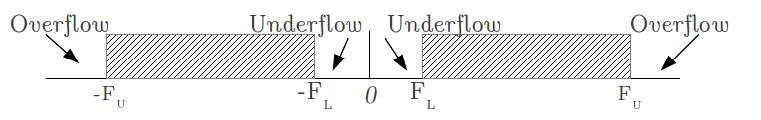
\includegraphics[scale=0.4]{./conj_F.jpg}
  \end{center}
  \caption{N\'umeros de punto flotante $\mathbb{F}(\beta, t, L, U )$.}
  \label{nums_flot}
  \end{figure}  
\end{frame}
%%%%%
\begin{frame}
\frametitle{Forma Normalizada de un N\'umero}
Sea el conjunto de punto flotante $\mathbb{F}$ con par\'ametros $\beta=2$(Binario), $t =3$ , $L = -2$, $U
=2$. Tal conjunto F tiene
$$
2(2-1)2^3-1(2-(-2)+1)+1=41
$$
n\'umeros diferentes (incluyendo el cero), en este caso, las mantisas ser\'ian $(0.100)_2$, $(0.101)_2$, $(0.110)_2$ y
$(0.111)_2$ los cuales son la representaci\'on en base dos de los n\'umeros reales $\frac{1}{2}$, $\frac{5}{8}$,
$\frac{3}{4}$ y $\frac{7}{8}$ respectivamente, el total de n\'umeros de m\'aquina aparecen en la siguiente tabla
\end{frame}
%%%%%
\begin{frame}
\begin{table}[!ht]
  \scriptsize{
\begin{center}
  \begin{tabular}{|c||c||c||c||c|}\hline
  -2  & -1 & 0 & 1 & 2\\\hline\hline
  $(0.100)_2\times2^{-2}$ & $(0.100)_2\times2^{-1}$ & $(0.100)_2\times2^{0}$ & $(0.100)_2\times2^{1}$ &
$(0.100)_2\times2^{2}$\\\hline
  $(0.101)_2\times2^{-2}$ & $(0.101)_2\times2^{-1}$ & $(0.101)_2\times2^{0}$ & $(0.101)_2\times2^{1}$ &
$(0.101)_2\times2^{2}$\\\hline
  $(0.110)_2\times2^{-2}$ & $(0.110)_2\times2^{-1}$ & $(0.110)_2\times2^{0}$ & $(0.110)_2\times2^{1}$ &
$(0.110)_2\times2^{2}$\\\hline
  $(0.111)_2\times2^{-2}$ & $(0.111)_2\times2^{-1}$ & $(0.111)_2\times2^{0}$ & $(0.111)_2\times2^{1}$ &
$(0.111)_2\times2^{2}$\\\hline
 \end{tabular}
 \caption{N\'umeros binarios de $\mathbb{F}(2,3,-2,2)$}\end{center}}
\end{table}
\end{frame}
%%%%%
\begin{frame}
\frametitle{Forma Normalizada de un N\'umero}
\begin{itemize}
 \item<1-> Los 41 n\'umeros de m\'aquina de este conjunto son los siguientes:
 $$
 \begin{array}{l}
 \displaystyle 0, \pm\frac{4}{32}, \pm\frac{5}{32}, \pm\frac{6}{32}, \pm\frac{7}{32}, \pm\frac{8}{32}, \pm\frac{10}{32},
 \pm\frac{12}{32}, \pm\frac{14}{32}, \pm\frac{16}{32}, \pm\frac{20}{32}, \pm\frac{24}{32},
 \pm\frac{28}{32},\\ 
 \displaystyle\pm\frac{32}{32}, \pm\frac{40}{32}, \pm\frac{48}{32}, \pm\frac{56}{32}, \pm\frac{64}{32},
 \pm\frac{80}{32}, \pm\frac{96}{32},  \pm\frac{112}{32}
 \end{array}
 $$
 
 \begin{figure}[ht]
 \begin{center}
   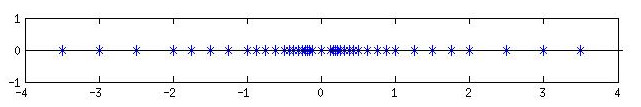
\includegraphics[scale=0.45]{./conj_F_ejem.jpg}
 \end{center}
 \caption{N\'umeros de punto flotante $\mathbb{F}(2, 3, -2, 2 )$.}
 \label{nums_flot_recta_real}
 \end{figure}
\end{itemize}
\end{frame}
%%%%%
\begin{frame}
  \frametitle{Forma Normalizada de un N\'umero}
  \begin{itemize}
   \item<1-> La combinaci\'on aritm\'etica usual $+$, $-$, $\times$, $\div$ de dos n\'umeros de punto flotante no siempre produce un n\'umero de punto flotante. 
   \item <2-> Supongamos que $fl(x)$, $fl(y) \in \mathbb{F}$. Veamos, como ejemplo, que la suma usual
   $fl(x)+fl(y)$ no necesariamente ser\'a un n\'umero en $\mathbb{F}$. Sea el conjunto $\mathbb{F}$ dado en el ejemplo: $fl(x) =5/32 \in \mathbb{F}$, $fl(y) =48/32 \in \mathbb{F}$, sin embargo $fl(x)+fl(y) =
   5/32 + 48/32 = 53/32 \notin \mathbb{F}$.
   \item Las operaciones aritm\'eticas que realiza un computador no corresponden de forma exacta con las operaciones usuales. El estudio de lo que ocurre realmente es dif\'icil de realizar y en todo caso depende de la m\'aquina que se est\'e
   utilizando.
  \end{itemize}
\end{frame}
%%%%%
\begin{frame}
   \frametitle{Forma Normalizada de un N\'umero}
   \begin{itemize}   
   \item Denotando por $\oplus,\ominus,\otimes,\oslash$ las operaciones de suma, resta, multiplicaci\'on y divisi\'on de la m\'aquina. Se definen estas operaciones por:
   \begin{block}{} 
   $$
   \begin{array}{lll}
    x \oplus y & = & fl(fl(x) + fl(y))\\
    x \ominus y & = & fl(fl(x) - fl(y))\\
    x \otimes y & = & fl(fl(x) \times fl(y))\\
    x \oslash y & = & fl(fl(x) / fl(y))\\
   \end{array}
   $$
   \end{block}
   \end{itemize}
\end{frame}
%%%%
\frame{
\frametitle{Ejercicios:}
 Asumiendo $\beta = 10$, $t = 3$, $L = -3$, $U = 4$, y la aritm\'etica es truncada. Obtener los 
valores de:
 
 \begin{itemize}
  \item $fl(0.00009)$
  \item $fl(3.146)$
  \item $fl(9996)$
  \item $fl((100.0 + 0.61) + 0.61)$ y $fl(100.0 + (0.61 + 0.61))$
  \item $fl(2.34 \times (5.67 + 8.90))$ y $fl((2.34 \times 5.67) + (2.34 \times 8.90))$
 \end{itemize}
}
%%%%%%
\frame
{
  \frametitle{Unidad de Precisi\'on o Redondeo} 
  \begin{itemize}
    \item<1-> En la representaci\'on en punto flotante con $n$ d\'igitos en base $\beta$ y exponente $e$, el error relativo en la
    representaci\'on de un n\'umero real $x$, $x\neq0$ es estimado por:     
    $$
    \left|\frac{x-fl(x)}{x}\right|\leq \mu = \left\{\begin{array}{ll}
      \beta^{1-n} & \mbox{ si se trunca}\\
      \frac{1}{2}\beta^{1-n} & \mbox{ si se redondea}
      \end{array}
    \right.
    $$     
    \item<2->El n\'umero $\mu$ (error de redondeo unitario) es una caracter\'istica de la m\'aquina, de su sistema operativo y de la manera en que efect\'ua los c\'alculos. 
    \item<3-> El \'epsilon de la m\'aquina es importante porque caracteriza la precisi\'on de la m\'aquina, sirve adem\'as como criterio de parada de los algoritmos.
  \end{itemize}
}
%%%%%
\begin{frame}
  \frametitle{Unidad de Precisi\'on o Redondeo} 
  \begin{itemize}
    \item Otra definici\'on de $\mu \approx \epsilon$ (\'Epsilon de la m\'aquina): $\epsilon$ es el m\'as peque\~no n\'umero positivo de la forma $\epsilon = 2^{-k}$ tal que:
    $$
    1.0 + \epsilon \neq 1.0 \mbox{  en la m\'aquina}
    $$
    \item<2-> $\epsilon = 2^{-n}$ donde $n$ es la precisi\'on de la m\'aquina. Lo que sucede es que en la aritm\'etica de la m\'aquina llega un momento en que:    
    $$
    fl(1.0 + 2^{-k}) = 1.0
    $$    
  \end{itemize}
\end{frame}
%%%%
\frame
{
  \frametitle{Unidad de Presici\'on o Redondeo.}
  Algoritmo para calcular $\epsilon$
  \begin{itemize}
  \item<1->[1.] $s=1$
  \item<2->[2.] para $k=1,2,\ldots,100$ hacer
  \item<3->[3.] \qquad $s= s*0.5$
  \item<4->[4.] \qquad $t=s+1.0$
  \item<5->[5.] \qquad si ($t<=1.0$) entonces
  \item<6->[6.] \qquad\qquad $s=2.0*s$
  \item<7->[7.] \qquad\qquad salida($k-1$,$s$)
  \item<8->[8.] \qquad\qquad parar
  \item<9->[9.] \qquad fsi
  \item<10->[10.] fpara
  \end{itemize}
}
%%%%%
\section{Propagaci\'on del Error.}
\frame
{
  \frametitle{Propagaci\'on del Error.}
  \begin{itemize}
    \item<1-> Es importante estudiar la propagaci\'on del error en los c\'alculos, ya que los errores se propagan y amplifican al realizar operaciones con dichos datos, hasta el punto de que puede suceder que el resultado carezca de significado.
    \item<2-> Con el proposito de ilustrar esta situaci\'on, seguidamente se calcula la diferencia entre los n\'umeros
    $$
    \begin{array}{l}
     a= 0.276435\\
    b=0.2756
    \end{array}
    $$
    \uncover<3->{Si los c\'alculos se realizan en base diez, punto flotante, redondeo correcto a tres d\'igitos de mantisa, los valores aproximados a dichos n\'umeros y el error relativo cometido es
    $$
    \begin{array}{lcl}
     \tilde a= 0.276 &  & |r_a|=1.57\times10^{-3}\\
    \tilde b=0.276 &  & |r_b|=1.45\times10^{-3}
    \end{array}
    $$}
  \end{itemize}
}
%%%%
\frame
{\frametitle{Propagaci\'on del Error}
\begin{itemize}
  \item Si ahora se calcula la diferencia entre los valores exactos y la diferencia entre los aproximados se obtiene
  $$
  \begin{array}{l}
   a-b= 0.000835\\
  \tilde a-\tilde b=0.0
  \end{array}
  $$
  \uncover<2->{
  \item<2->Debe observa que el error relativo de la diferencia aproximada es del 100\%. Este ejemplo, extraordinariamente sencillo, pone de manifiesto como el error de redondeo de los datos se ha amplificado al realizar una \'unica operaci\'on, hasta generar un resultado carente de significado.
  }
\end{itemize}
}
%%%%
\frame
{
\frametitle{Propagaci\'on del Error en la Suma}

Denotando por $x$ e $y$ los valores exactos de dos n\'umeros y por $\tilde x$ e $\tilde y$ sus valores aproximados. As\'i mismo, los errores absolutos y relativos de estas cantidades se denotar\'an por $E_x$, $E_y$, $r_x$, $r_y$, respectivamente. Si se representa por $s = x + y$ al valor exacto de la suma y por $\tilde s = \tilde x + \tilde y$ su valor aproximado, entonces el error absoluto de la suma es
$$
E_s = s -\tilde s = (x + y) - (\tilde x + \tilde y) = E_x + E_y
$$

El error relativo vale
$$
r_s = \frac{E_s}{s} = \frac{E_x+E_y}{x+y} = \frac{x}{x+y}r_x + \frac{y}{x+y}r_y
$$
}

\frame
{
\frametitle{Propagaci\'on del Erroren la Resta}

La deducci\'on para la propagaci\'on del error mediante la resta es muy parecida a la anterior. Si se representa por $r = x - y$ al valor exacto de la resta y por $\tilde r =\tilde x -\tilde y$ su valor aproximado, entonces el error absoluto es
$$
E_r = r -\tilde r = (x - y) - (\tilde x - \tilde y) = E_x - E_y
$$

El error relativo vale
$$
r_r = \frac{E_r}{r} = \frac{E_x-E_y}{x-y} = \frac{x}{x-y}r_x - \frac{y}{x-y}r_y
$$
}
%%%%
\frame
{
\frametitle{Propagaci\'on del Error en el Producto}
Si se representa el producto de dos n\'umeros exactos mediante $p = xy$ y el valor aproximado del producto por $\tilde p = \tilde x\tilde y$, el error absoluto del producto se puede calcular como

\begin{eqnarray}
\nonumber E_p &=& p -\tilde p = (xy) - (\tilde x \tilde y) = xy - (x-E_x) (y- E_y)\\
\nonumber &=& x E_y + y E_x - E_x E_y \approx xE_y + yE_x
\end{eqnarray}


El error relativo vale
$$
r_p = \frac{E_p}{p} = \frac{xE_y+yE_x-ExEy}{xy} = r_x+r_y+r_xr_y \approx r_x+r_y
$$
}
%%%%
\frame
{
\frametitle{Propagaci\'on del Error en la Divisi\'on}

Si se representa el cociente de dos n\'umeros exactos mediante $d = x/y$ y el valor aproximado del producto por $\tilde d = \tilde x/\tilde y$, el error absoluto del cociente se puede calcular como

\begin{eqnarray}
\nonumber E_d &=& d -\tilde d = \frac{x}{y} - \frac{\tilde x}{\tilde y} =\frac{x}{y} - \frac{x-Ex}{y-Ey}\\
\nonumber &=& \frac{yE_x-xE_y}{y(y-Ey)} \approx \frac{yE_x-xE_y}{y^2}
\end{eqnarray}


El error relativo vale
$$
r_d = \frac{E_d}{d} = \frac{\frac{yE_x-xE_y}{y(y-Ey)}}{\frac{x}{y}} = \frac{yE_x-xE_y}{x(y-E_y)} =  \frac{r_x-r_y}{1-r_y} \approx r_x-r_y
$$
}
%%%%
\frame
{
\frametitle{Propagaci\'on del Error en una Funci\'on}

Sea $z = f(x)$ la imagen mediante la funci\'on $f$ del valor exacto de un n\'umero $x$ y sea $\tilde z = f(\tilde x)$ la imagen de su valor aproximado. Entonces, el error absoluto de la imagen es

\begin{eqnarray}
\nonumber E_z &=& f(x) -f(\tilde x) = f(x) - f(x-E_x)\\
\nonumber &=& f(x) - \left[f(x)-f'(x)E_x+f''(x)\frac{E_x^2}{2!}-f'''(x)\frac{E_x^3}{3!}+\cdots\right]\\
\nonumber &=& f'(x)E_x-f''(x)\frac{E_x^2}{2!}+f'''(x)\frac{E_x^3}{3!}-\cdots \approx f'(x)E_x
\end{eqnarray}

El error relativo vale
%\small 
$$
r_z = \frac{E_z}{z} = \frac{f'(x)E_x-f''(x)\frac{E_x^2}{2!}+f'''(x)\frac{E_x^3}{3!}-\cdots}{f(x)}  \approx  x\frac{f'(x)}{f(x)}r_x 
$$
}
%%%%%
\section{Estabilidad en el An\'alisis Num\'erico}
\frame
{
  \frametitle{P\'erdida de Cifras Significativas.}
\begin{itemize}

  \item<1-> Este tipo de situaci\'on se da cuando alg\'un c\'alculo envuelve la resta de dos cantidades similares \'o en el c\'alculo de un n\'umero por medio de una sumatoria donde el resultado es menor que los t\'erminos de la sumatoria los cuales alternan en signo.

  \item<2-> Por ejemplo: Sea $f(x)=\sqrt{x+1}-\sqrt{x}$ para $x$ grande. Suponemos que trabajamos con seis cifras significativas. Veamos el caso de calcular $f(100)$.

  $\sqrt{100}=10.000 \qquad \sqrt{101}=10.0499$

  Calculamos $f(100) = \sqrt{101}-\sqrt{100} = 0.499000\times10^{-1}$. El valor exacto a seis cifras de $f(100)$ es $0.498756\times10^{-1}$
\end{itemize}

}
%%%%
\frame
{
  \frametitle{P\'erdida de Cifras Significativas.}
\textquestiondown C\'ual fu\'e el problema? Se restaron cantidades similares. En este caso se puede evitar restando cantidades similares si se reescribe $f(x)$ (racionalizando) como:
$$
f(x)=\frac{1}{\sqrt{x+1}+\sqrt{x}}
$$  

$$
f(100)=\frac{1}{10.000 +10.0499 } = \frac{1}{20.0499} = 0.498756\times10^{-1}
$$
}
%%%%
\frame
{
  \frametitle{Condicionamiento y Estabilidad.}

  \begin{itemize}
    \item<1-> La condici\'on de un problema o de una funci\'on es la medida de la sensibilidad de esa funci\'on a peque\~nos cambios en sus par\'ametros.
    \item<2-> Una funci\'on est\'a bien condicionada si peque\~nos cambios en los par\'ametros inducen solo un cambio peque\~no en el comportamiento de la funci\'on; de otro modo, est\'a mal condicionada.
  \end{itemize}
}
%%%%
\frame
{
  \frametitle{Condicionamiento y Estabilidad.} 
  \begin{itemize}
    \item<1-> Supongamos que se quiere calcular la integral
    \begin{block}{}
    $$
      E_n = \int_0^1x^ne^{x-1}dx, \qquad n=1,2,\ldots
    $$  
    \end{block}
    \item<2->Usando integraci\'on por partes
    \begin{block}{}
      $$
      \int_0^1x^ne^{x-1}dx = \displaystyle \left. x^ne^{x-1}\right|_0^1 - \int_0^1nx^{n-1}e^{x-1}dx
      $$
    \end{block}
    o bien 
    \begin{block}{}
    $$
    E_n = 1 - nE_{n-1}, \qquad n=2,\ldots
    $$
    \end{block}
  \end{itemize}
}
%%%%
\frame
{
  \frametitle{Condicionamiento y Estabilidad.}
  \begin{itemize}
    \item<1-> Donde $E_1=e^{-1}$
    \item<2-> Supongamos que se comienza el proceso iterativo con $\tilde E_1 = E_1 + \varepsilon$ y efectuamos todas las operaciones aritm\'eticas en forma exacta. Entonces,
\begin{block}{}
\begin{align}
 &\nonumber \tilde E_2 = 1 - 2\tilde E_1 = 1 - 2E_1 - 2\varepsilon = E_2 - 2\varepsilon\\ 
 &\nonumber \tilde E_3 = 1 - 3\tilde E_2 = 1 - 3E_2 + 6\varepsilon = E_3 + 3!\varepsilon\\
 &\nonumber \tilde E_4 = 1 - 4\tilde E_3 = 1 - 4E_3 - 24\varepsilon = E_4 - 4!\varepsilon\\
 &\nonumber \vdots\\
 &\nonumber \tilde E_n = E_n \pm n!\varepsilon
\end{align}
\end{block}
\end{itemize}
}
%%%%
\frame
{
  \frametitle{Condicionamiento y Estabilidad.} 
  \begin{itemize} 
    \item<1-> Un peque\~no cambio en el valor inicial $E_1$ origina un gran cambio en los valores posteriores de $E_n$.
    \item<2-> De hecho, en este caso, el efecto es devastador: puesto que los valores exactos de $E_n$ decrecen conforme $n$ aumenta, y a partir de cierto $n$ el error ser\'a tan o m\'as grande que el valor a estimar. 
    \item<3-> Claramente, el algoritmo recursivo propuesto es num\'ericamente inestable.
  \end{itemize}
}
%%%%
\frame
{
  \frametitle{Condicionamiento y Estabilidad.}
  \begin{itemize}
    \item<1-> Para evitar el efecto devastador del error, se puede usar una f\'ormula recursiva que permita calcular aproximaciones a $E_n$ a partir de aproximaciones a $E_{n-1}$.
    \item<2->Consid\'erese la f\'ormula recursiva escrita en forma inversa,
    \begin{block}{}
      $$
      E_{n-1} = \frac{1 - E_n}{n}, \qquad n=\ldots,N,N-1,\ldots,3,2,1
      $$
    \end{block}
    \item<3-> Si se conoce una aproximaci\'on $\tilde E_N$ a $E_N$ para alg\'un $N$, entonces la f\'ormula anterior permitir\'ia calcular aproximaciones a $E_{N-1}, E_{N-2},\ldots , E_1$.
  
  \end{itemize}
}
%%%%
\frame
{
  \frametitle{Condicionamiento y Estabilidad.}
  \begin{itemize}
    \item<1->Para determinar la estabilidad del proceso
recursivo considerese, en forma an\'aloga a lo anterior, que $\tilde E_N = E_N + \varepsilon$, entonces
\begin{block}{}
  \begin{align}
    & \nonumber \tilde E_{N-1} = \frac{1- \tilde E_N}{N} = \frac{1-E_N}{N} - \frac{\varepsilon}{N} = E_{N-1} -
   \frac{\varepsilon}{N}\\
    & \nonumber \tilde E_{N-2}  = E_{N-2} + \frac{\varepsilon}{N(N-1)}\\
    & \nonumber \vdots\\
    & \nonumber \tilde E_1 = E_1 \pm \frac{\varepsilon}{N!}
   \end{align}     
\end{block}
\end{itemize}
}
%%%%
\frame{
  \frametitle{Condicionamiento y Estabilidad.}
  \begin{itemize}
    \item<1-> Se observa que el error introducido en $E_N$ es r\'apidamente reducido en cada paso. M\'as a\'un, la
magnitud del error tiende a ser mucho menor respecto del valor a estimar. 
\item<2-> Esto \'ultimo permite que, a\'un con una pobre
aproximaci\'on $\tilde E_N$ para alg\'un $N$ suficientemente grande, se puede obtener una aproximaci\'on precisa para el valor $E_n$ de inter\'es.
\item<3->Para obtener un valor inicial, n\'otese que:
\begin{block}{}
$$
E_n = \int_0^1x^ne^{x-1}dx  \leq \int_0^1 x^ndx = \displaystyle\left.\frac{x^{n+1}}{n+1}\right|_0^1 = \frac{1}{n+1}
$$
\end{block}
\end{itemize}
}
%%%%
\frame{
  \frametitle{Condicionamiento y Estabilidad.}
  \begin{itemize}
    \item<1-> Por tanto, $E_n$ tiende a cero cuando $n$ tiende a $\infty$. Por ejemplo, si aproximamos $E_{20}$ por cero y usamos este valor para empezar, como mucho cometemos un error de $\frac{1}{21}$.
\item<2-> Este error es multiplicado por $\frac{1}{20}$ al
calcular $E_{19}$, y el error en $E_{19}$ es a lo m\'as $\left(\frac{1}{21}\right)\left(\frac{1}{20}\right) \approx
0.0024$. 
\item<3-> Al llegar a $E_{15}$, el error inicial ha sido reducido a menos de $4 \times 10^{-8}$, que ya es menor que el error de redondeo.
\end{itemize}
}
\end{document}